\begin{tikzpicture}[>=latex, scale=1]
	\definecolor{blueT}		{RGB}{0,0,220};
	\def\re0{7.5-0.6*15/2.6};
	\def\im0{0};

	\node at (7.8,4.8) {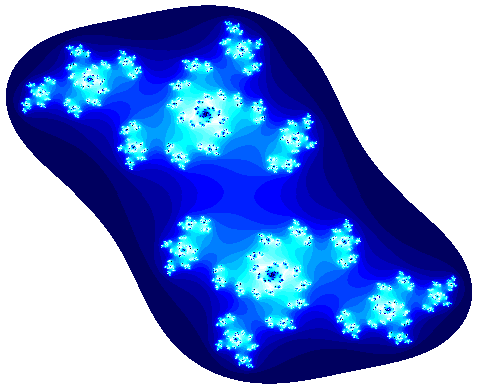
\includegraphics[width=5.5cm]{apfel/pic/julia005j072.png}};
	\node at (7.8,-4.8) {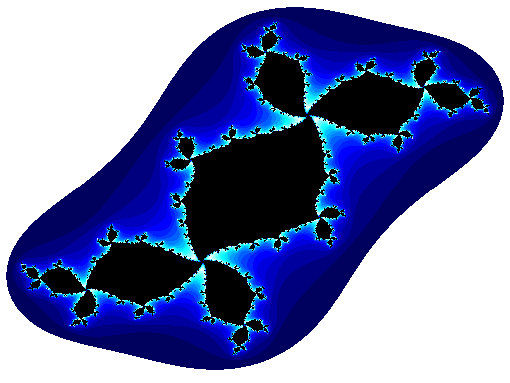
\includegraphics[width=5.5cm]{apfel/pic/julia-015j-075.png}};
	\node at (-2.8,4.2) {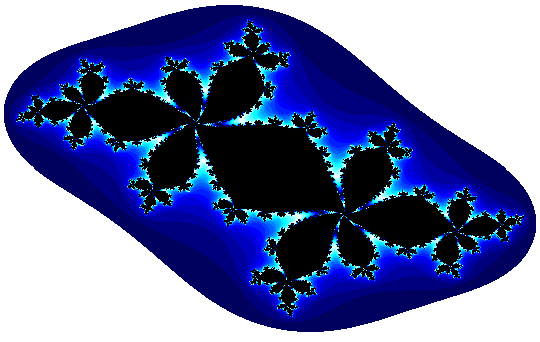
\includegraphics[width=5.5cm]{apfel/pic/julia-05j055.png}};
	\node at (-3.2,-4.2) {
\includegraphics[width=7cm]{apfel/pic/julia-075j-015.png}};

	\node at (0,0) {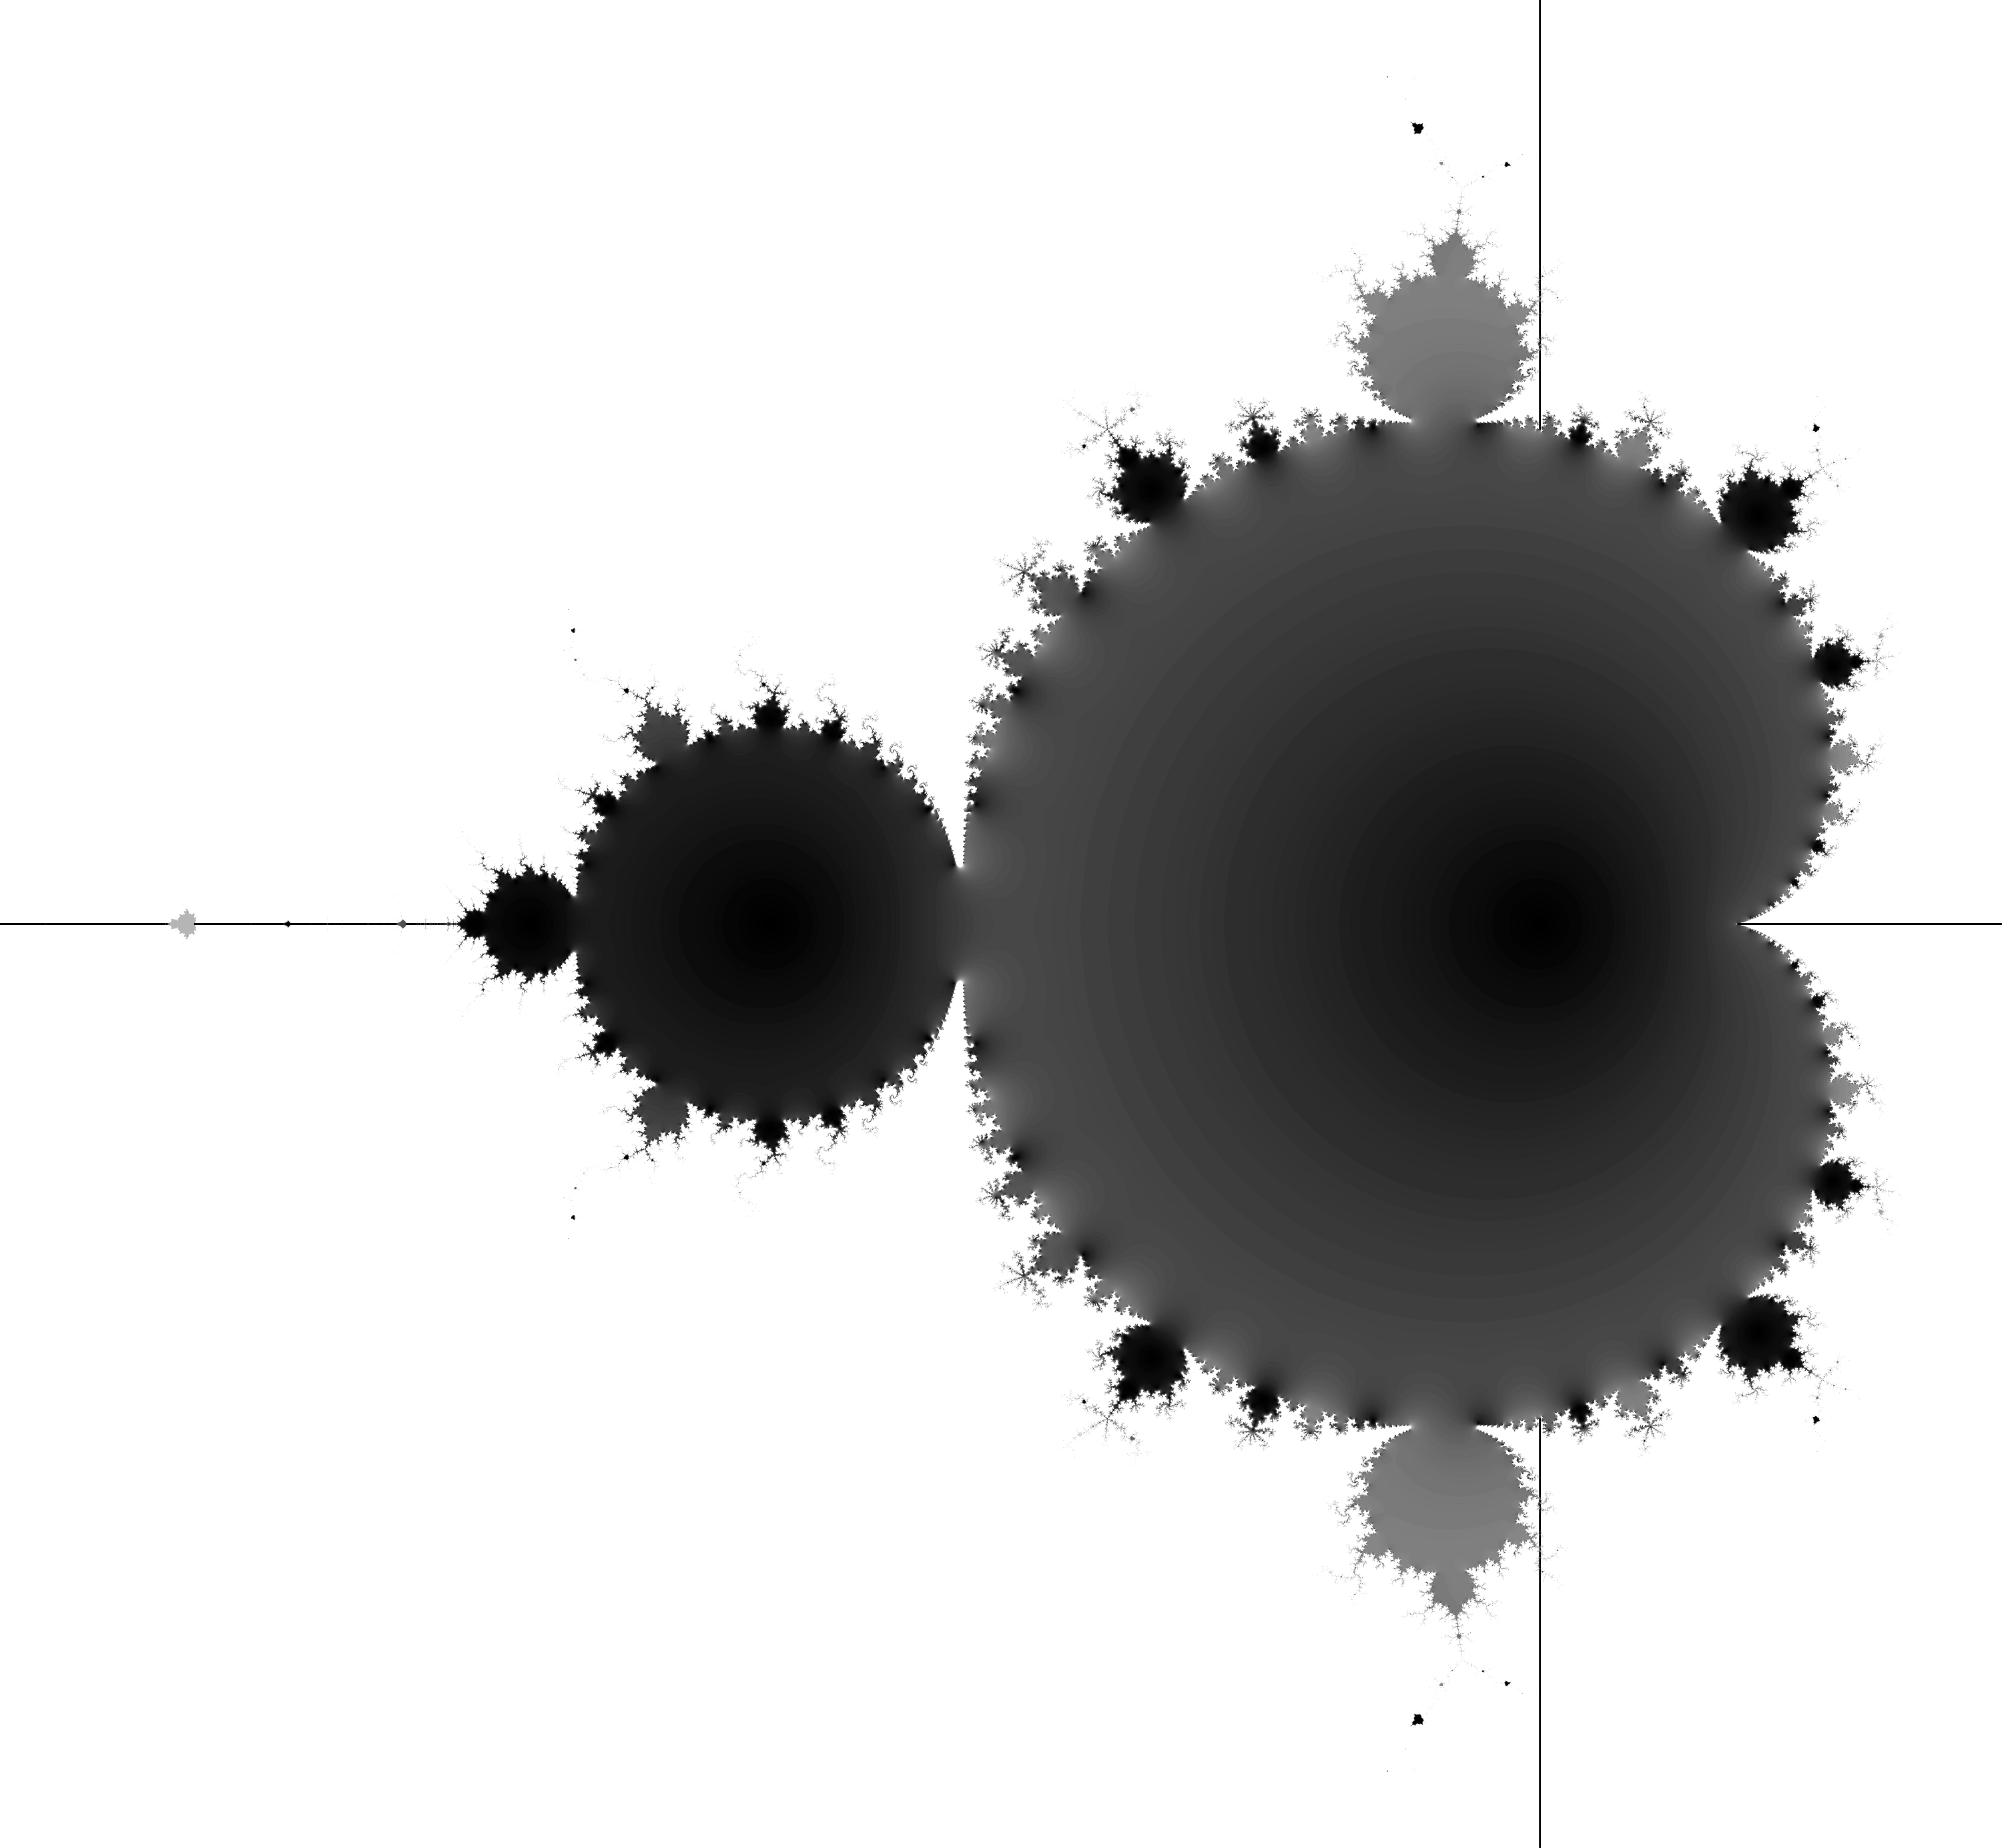
\includegraphics[width=15cm]{apfel/pic/apfelroman0251200koordinatenkomp.png}};
	\draw[->,line width=2](\re0+0.6*15/2.6-0.1,\im0)--++(0.15,0)node[below]{\large Re};
	\draw[->,line width=2](\re0,\im0+1.2*15/2.6-0.1)--++(0,0.15)node[right]{\large Im};


	\draw[blueT, fill] (\re0+0.05*15/2.6,\im0+0.72*15/2.6) circle (4pt);
	\draw[blueT, line width=1.5] (\re0+0.05*15/2.6,\im0+0.72*15/2.6) ++(0.2,0.04)--++(1.6,0.3);

	\draw[blueT, fill] (\re0-0.15*15/2.6,\im0-0.75*15/2.6) circle (4pt);
	\draw[blueT, line width=1.5] (\re0-0.15*15/2.6,\im0-0.75*15/2.6) ++(0.2,-0.04)--++(1.6*1.45,-0.3*1.45);

	\draw[blueT, fill] (\re0-0.5*15/2.6,\im0+0.55*15/2.6) circle (4pt);
	\draw[blueT, line width=1.5]  (\re0-0.5*15/2.6,\im0+0.55*15/2.6) ++(-0.2,0.04)--++(-1.6*0.65,0.3*0.65);

	\draw[blueT, fill] (\re0-0.75*15/2.6,\im0-0.15*15/2.6) circle (4pt);
	\draw[blueT, line width=1.5] (\re0-0.75*15/2.6,\im0-0.15*15/2.6) ++(-0.06,-0.19)--++(-0.3*1.25,-1.6*1.25);
\end{tikzpicture}
